\chapter{研究目的}\label{ch:purpose}
%
\section{分類対象}
今回対象とする情報は,SNS上で投稿された画像つきで発信されたニュースである.
そのなかでも,正しいニュースを発信していたもの,フェイクニュースを発信していたもの,ジョークニュースを発信していたものが対象となる.
それぞれの例を今回扱ったデータセットから抜粋したものが以下の図\ref{fig:examples}である.

\begin{figure}[ht]
    \centering
    \begin{subfigure}[b]{0.4\textwidth}
        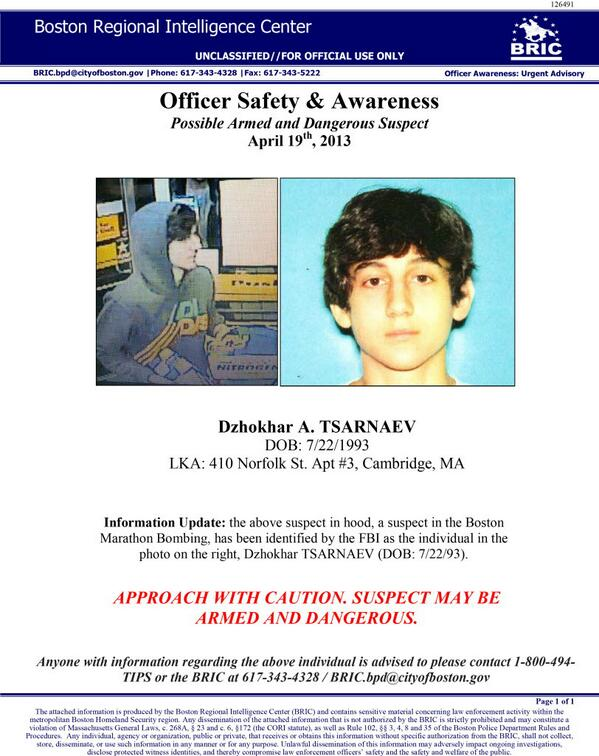
\includegraphics[height=5cm]{images/real_example_boston.jpg}
        \caption{Boston RIC released this flier showing at large suspect Dzhokhar Tsarnaev. He may be armed \& dangerous}
        \label{fig:real}
    \end{subfigure}
    \hfill % separation between the subfigures
    \begin{subfigure}[b]{0.57\textwidth}
        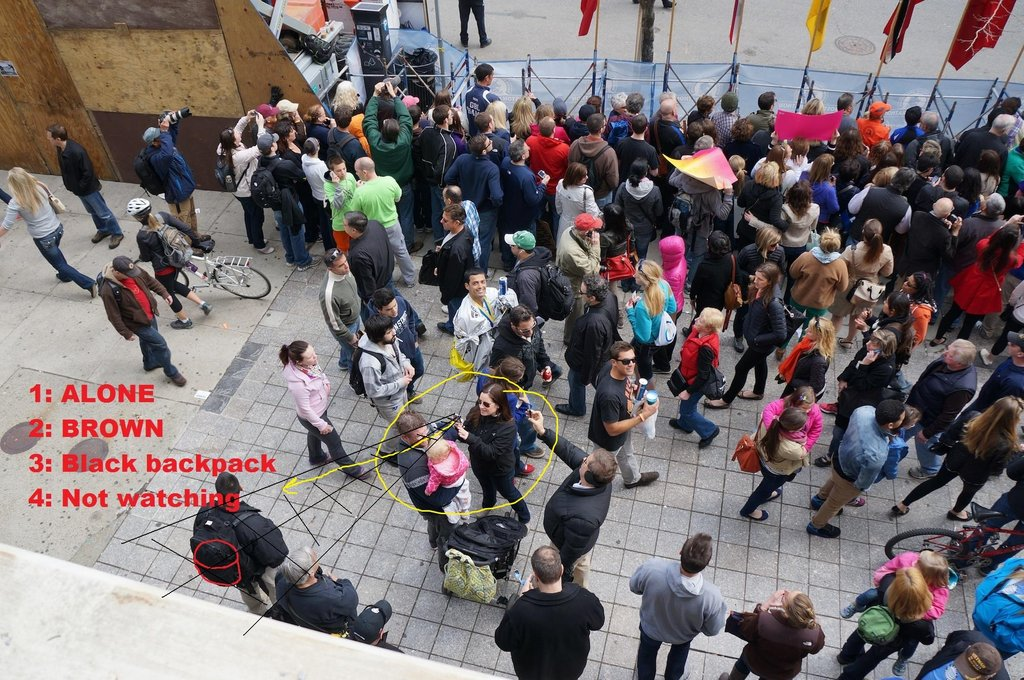
\includegraphics[height=5cm]{images/humor_example_boston.jpg}
        \caption{The detail of these photos used to identify the Boston Marathon bombing suspect is bananas…}
        \label{fig:humor}
    \end{subfigure}
    \bigskip 
    \centering
    \begin{subfigure}[b]{\textwidth}
        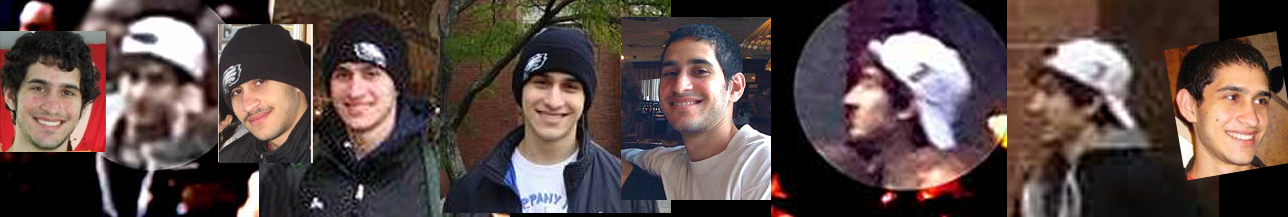
\includegraphics[width=\textwidth]{images/fake_example_boston.jpg}
        \caption{Reddit is on to something... Boston Bomber \#2 sure looks like missing student Sunil Tripathi. }
        \label{fig:fake}
    \end{subfigure}
    \caption{当研究で扱う3カテゴリの投稿例: (a)正しいニュース,(b)ジョークニュース,(c)フェイクニュース}
    \label{fig:examples}
\end{figure}

いずれも2013年に発生したボストンマラソン爆弾テロ事件に関してTwitter上で投稿されたものであった.
図\ref{fig:real}は実際にボストン市傘下組織が作成した被疑者の情報をChicago Sun-TimesがTwitterに投稿したもの,
図\ref{fig:humor}はテロ後にRedditや4chanの有志によって実行犯の調査が行われた件に対して
``bananas''と茶化すような言葉を投げかけているもの,
図\ref{fig:fake}は実際に上記掲示板上で実行犯の調査が行われた結果,
全くの別人を槍玉に挙げているものである.

実際に,ボストンマラソン後ではインターネット上で盛んに犯人探しが行われた結果,
事件前に行方不明になっていたスニル・トリパティ(Sunil Tripathi)さんが犯人として扱われ,
更にその後一般報道メディアによってトリパティさんの家族に取材が行われるなど,
フェイクニュースが実害として現実になった\cite{gray_2013}.
これを受け,Redditでは実際に犯人探しの過熱で無関係の個人とその家族に迷惑をかけたとして謝罪した\cite{laird_2013}.

%
\section{達成目標}
当研究では,上記対象を正確に3カテゴリへ分類する手法を構築することを目標としている.
具体的には,入力として画像と文章を持ち,それに対してどのカテゴリが該当するかを出力する手法となる.
ジョークニュースとフェイクニュースを完全に区別することで,
センセーショナリズムによる影響を最小限に留め,
なおかつ高い精度を維持することを目指すことにする.

当研究を更に発展させると,SNS上でフェイクニュースに該当する記事に対してユーザへ警告を出したり,
ジョーク記事の場合はそれを知らせる追加情報を与えたりするユーザエージェントを開発することへ繋げられる.
また繰り返しフェイクニュースを発信するユーザがいる場合は,
運営側へアカウント停止等のペナルティを迅速に進言するエージェント開発にも発展可能である.

%